\documentclass[11pt]{article}
\usepackage[margin=1in]{geometry}
\usepackage{amsmath,amssymb,amsthm}
\usepackage{tikz}
\usetikzlibrary{positioning}
\newtheorem{theorem}{Theorem}
\theoremstyle{definition}
\newtheorem*{definition*}{Definition}
\newenvironment{exambox}
  {\par\medskip\noindent\begin{center}\begin{minipage}{0.92\textwidth}%
   \hrule height 1pt \vspace{4pt}\noindent\textbf{$\bigstar$ EXAM PRIORITY.} }
  {\vspace{4pt}\hrule height 1pt \end{minipage}\end{center}\medskip}
\title{CSEN 19 -- Trees and Spanning Trees (June 5, 2026)}
\date{}
\author{}
\begin{document}
\maketitle

\section*{Trees: Definition and Characterization}

Recall that a \emph{tree} is a connected, acyclic graph.  An acyclic graph
(not necessarily connected) is called a \emph{forest}; each connected
component of a forest is a tree.  The figure below shows a forest with
three components.

\begin{center}
\begin{tikzpicture}
  [every node/.style={circle, draw, minimum size=6pt, inner sep=0pt}]
  % Component 1: a small tree on 3 vertices
  \node (a) at (0,   0.9) {};
  \node (b) at (0.8, 0)   {};
  \node (c) at (0,   0)   {};
  \draw (a)--(b) (a)--(c);
  % Component 2: a path on 3 vertices
  \node (d) at (2.5, 1.0) {};
  \node (e) at (2.5, 0.3) {};
  \node (f) at (3.3, 0.3) {};
  \draw (d)--(e) (e)--(f);
  % Component 3: an isolated vertex
  \node (g) at (4.6, 0.6) {};
\end{tikzpicture}
\par\smallskip\small
A forest with three components (two non-trivial trees and one isolated vertex).
\end{center}

The central theorem of this lecture gives three equivalent ways to recognize
a tree.

\begin{theorem}[Characterization of Trees]
Let $G$ be a finite graph with $n$ vertices and $m$ edges.  The following
conditions are equivalent:
\begin{enumerate}
  \item[(1)] $G$ is connected and acyclic.
  \item[(2)] $G$ is connected and $m = n-1$.
  \item[(3)] $G$ is acyclic and $m = n-1$.
\end{enumerate}
\end{theorem}

We establish the cyclic chain $(1)\Rightarrow(2)\Rightarrow(3)\Rightarrow(1)$.

\begin{proof}[Proof of $(1)\Rightarrow(2)$]
Assume $G$ is connected and acyclic.  We induct on $n$.  For $n=1$,
$m=0=n-1$.  For $n\geq 2$, recall the longest-path argument from last
lecture: every finite tree has at least one \emph{leaf}, a vertex $v$ with
$\deg(v)=1$.  The subgraph $G-v$ is still connected and acyclic, so by
induction $G-v$ has $n-2$ edges.  Restoring $v$ adds exactly one edge, so
$m=(n-2)+1=n-1$.
\end{proof}

\begin{proof}[Proof of $(2)\Rightarrow(3)$]
Assume $G$ is connected and $m=n-1$.  Suppose for contradiction that $G$
contains a cycle.  Remove one edge $e$ from that cycle; since $e$ lies on
a cycle it is not a bridge, so $G-e$ remains connected.  If $G-e$ still
has a cycle, remove another edge, and so on.  Let $\widetilde{G}$ be the
result after removing $k\geq 1$ edges total.  Then $\widetilde{G}$ is
connected and acyclic, i.e.\ a tree on $n$ vertices, so by
$(1)\Rightarrow(2)$ it has $n-1$ edges.  But also
$|E(\widetilde{G})|=m-k=n-1-k$, giving
\[
  n-1 = n-1-k \implies k=0,
\]
which contradicts $k\geq 1$.  Hence $G$ is acyclic.
\end{proof}

\begin{proof}[Proof of $(3)\Rightarrow(1)$]
Assume $G$ is acyclic and $m=n-1$.  Let $G$ have $c$ connected components
$T_1,\ldots,T_c$.  Each component is acyclic and connected, hence a tree.
Summing edge counts:
\begin{align*}
  n-1 &= m \\
      &= \sum_{i=1}^{c}|E(T_i)|
       = \sum_{i=1}^{c}\bigl(|V(T_i)|-1\bigr) \\
      &= \sum_{i=1}^{c}|V(T_i)| - c = n-c.
\end{align*}
Therefore $c=1$, so $G$ is connected.
\end{proof}

\begin{exambox}
Know all three equivalent characterizations of a tree.  Be prepared to
reproduce both edge-counting arguments: the contradiction giving $k=0$ in
$(2)\Rightarrow(3)$, and the component-sum giving $c=1$ in
$(3)\Rightarrow(1)$.
\end{exambox}

\section*{Spanning Trees}

\begin{definition*}
Let $G$ be a connected graph.  A \emph{spanning tree} of $G$ is a subgraph
$T\subseteq G$ such that $T$ is a tree and $V(T)=V(G)$.
\end{definition*}

A spanning tree retains every vertex of $G$ but discards edges until no
cycle remains.  Below, the solid edges form a spanning tree of the graph
consisting of all (solid and dashed) edges.

\begin{center}
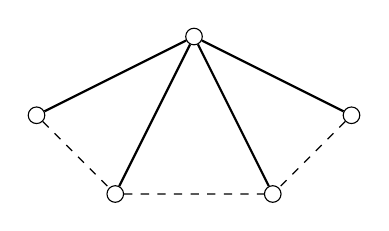
\begin{tikzpicture}
  [every node/.style={circle, draw, minimum size=6pt, inner sep=0pt}]
  \node (a) at (0, 1) {};
  \node (b) at (2, 2) {};
  \node (c) at (4, 1) {};
  \node (d) at (1, 0) {};
  \node (e) at (3, 0) {};
  % Spanning tree: b connected to all others (a star)
  \draw[thick] (b)--(a) (b)--(c) (b)--(d) (b)--(e);
  % Extra edges of G not in the spanning tree
  \draw[dashed] (a)--(d) (c)--(e) (d)--(e);
\end{tikzpicture}
\par\smallskip\small
Solid edges: spanning tree.  Dashed edges: remaining edges of $G$.
\end{center}

\begin{theorem}
Every connected graph $G$ has a spanning tree.
\end{theorem}

\begin{proof}
If $G$ is already a tree, take $T=G$.  Otherwise $G$ contains a cycle;
remove one edge from that cycle.  A cycle edge is not a bridge, so
connectivity is preserved.  Repeat until no cycle remains.  The resulting
subgraph $T$ is connected, acyclic, and spans $V(G)$, so $T$ is a spanning
tree of $G$.
\end{proof}

\begin{exambox}
Every connected graph has a spanning tree.  The proof is constructive:
repeatedly delete a cycle edge (connectivity is preserved at each step)
until the graph is acyclic.
\end{exambox}

\section*{A Non-Cut-Vertex Theorem}

A vertex $v$ is a \emph{cut vertex} of $G$ if $G-v$ is disconnected.  The
following theorem, proved using a spanning tree, guarantees that every
connected graph has at least one vertex that is not a cut vertex.

\begin{theorem}
Let $G$ be a connected graph with $n\geq 2$ vertices.  Then there exists a
vertex $v\in V(G)$ such that $G-v$ is connected.
\end{theorem}

\begin{proof}
Let $T$ be a spanning tree of $G$ and let $v$ be a leaf of $T$, i.e.\
$\deg_T(v)=1$ (every tree with $n\geq 2$ has at least two leaves).  The
subgraph $T-v$ is a tree on $n-1$ vertices, hence connected.  Since
$V(T-v)=V(G-v)$ and $E(T-v)\subseteq E(G-v)$, the graph $G-v$ contains
$T-v$ as a connected spanning subgraph, so $G-v$ is connected.
\end{proof}

The figure below illustrates the proof: $v$ (shaded) is a leaf of the
spanning tree; removing it leaves the remaining vertices connected.

\begin{center}
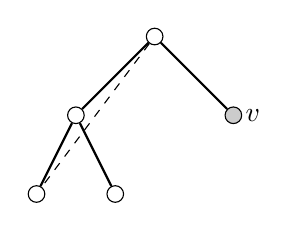
\begin{tikzpicture}[
  every node/.style={circle, draw, minimum size=6pt, inner sep=0pt},
  every label/.style={draw=none, fill=none, rectangle, inner sep=1pt}
]
  \node (r) at (1,    2)  {};
  \node (a) at (0,    1)  {};
  \node[fill=gray!40, label={right:$v$}] (v) at (2, 1) {};
  \node (c) at (-0.5, 0)  {};
  \node (d) at (0.5,  0)  {};
  \draw[thick] (r)--(a) (r)--(v) (a)--(c) (a)--(d);
  \draw[dashed] (r)--(c);
\end{tikzpicture}
\end{center}

\section*{Dominating Sets via Spanning Trees}

\begin{definition*}
Let $G$ be a graph.  A subset $D\subseteq V(G)$ is a \emph{dominating set}
of $G$ if every vertex $u\notin D$ has at least one neighbor in $D$.
\end{definition*}

\begin{theorem}
Every graph $G$ with $n\geq 2$ vertices has a dominating set of size at
most $\lfloor n/2\rfloor$.
\end{theorem}

\begin{proof}
It suffices to handle each connected component separately, so assume $G$ is
connected.  Let $T$ be a spanning tree of $G$.  Root $T$ at any vertex and
partition $V(G)$ by the parity of each vertex's depth:
\[
  A = \{\,v : \operatorname{depth}(v)\text{ is even}\,\},\qquad
  B = \{\,v : \operatorname{depth}(v)\text{ is odd}\,\}.
\]
Every vertex in $B$ has its parent (at even depth) in $A$, so every vertex
outside $A$ is adjacent to a member of $A$; thus $A$ is a dominating set.
By the symmetric argument, $B$ is also a dominating set.  Since
$|A|+|B|=n$, we have $\min(|A|,|B|)\leq\lfloor n/2\rfloor$.
\end{proof}

\section*{Trees Are Bipartite}

Because trees are acyclic, they contain no odd cycles.  By the
characterization of bipartite graphs (a graph is bipartite if and only if
it has no odd cycle), every tree is bipartite.  The bipartition is
precisely the even-depth/odd-depth partition used in the dominating-set
proof above.

\begin{exambox}
Trees are bipartite because they have no cycles.  Bipartiteness is a graph
isomorphism invariant: if one graph is bipartite and another is not, the
two graphs cannot be isomorphic.
\end{exambox}

\end{document}